% BB84 from end to end (notebook 53, Figure 1). Quantum stage: Alice picks a random bit a and a random basis (Z or X)
% and sends one of |0>, |1>, |+>, |->; Eve controls the quantum channel; Bob measures in a random basis and records b.
% Classical stage, over the public authenticated channel (Eve reads everything, cannot change anything): sifting
% (announce bases, keep matching rounds), parameter estimation (QBER Q on a random sample, abort if Q is too large),
% error correction (parity checks, about h(Q) bits revealed per key bit), privacy amplification (random hash k = G x).
% The result is the same secret key on both sides, of length about n [1 - 2 h(Q)] (Section 7).
\documentclass[tikz,border=6pt]{standalone}
\usepackage{amsmath,amssymb}
\usetikzlibrary{arrows.meta,positioning,calc}
\begin{document}
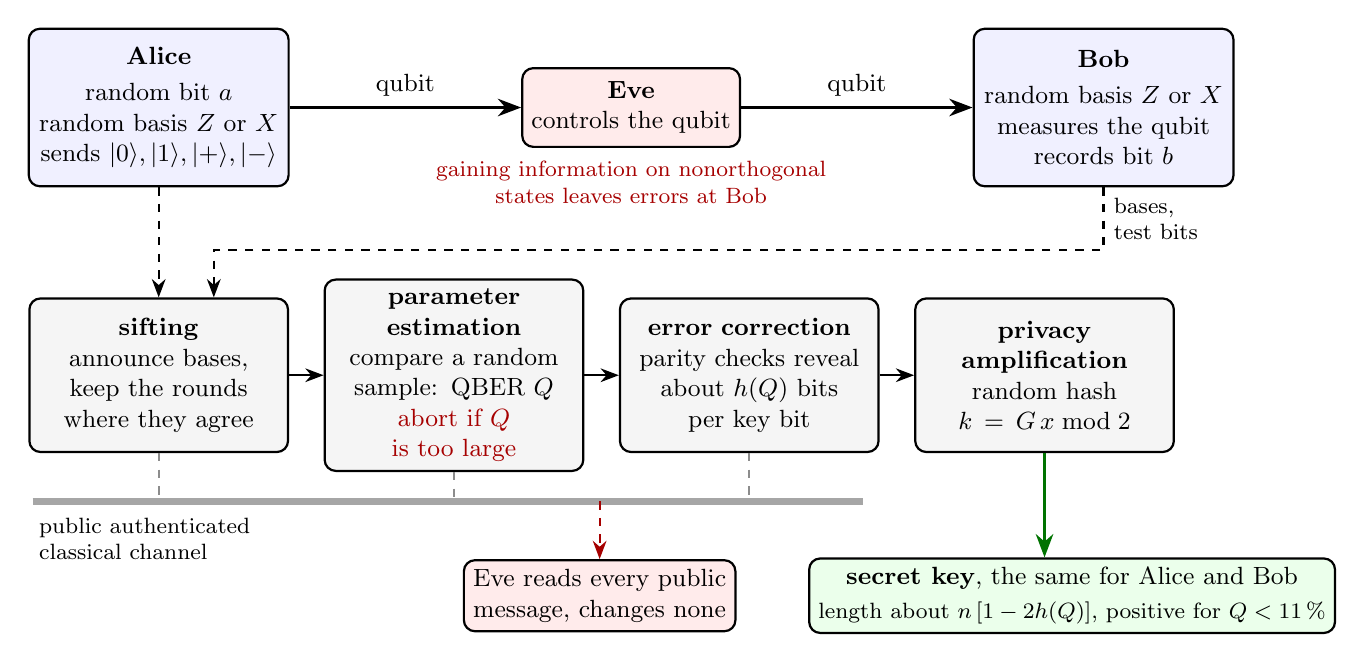
\begin{tikzpicture}[thick, >=Stealth, font=\small,
    party/.style={draw, rounded corners, fill=blue!6, minimum height=2.0cm, minimum width=3.3cm, align=center},
    adv/.style={draw, rounded corners, fill=red!8, minimum height=1.0cm, minimum width=2.4cm, align=center},
    stage/.style={draw, rounded corners, fill=black!4, minimum height=1.95cm, text width=3.05cm, align=center},
    keyb/.style={draw, rounded corners, fill=green!8, minimum height=0.9cm, minimum width=3.3cm, align=center}]
  % ---------------- quantum stage ----------------
    \node[party] (A) at (0,0)
       {\textbf{Alice}\\[2pt] random bit $a$\\ random basis $Z$ or $X$\\ sends $\vert0\rangle,\vert1\rangle,\vert{+}\rangle,\vert{-}\rangle$};
  \node[party] (B) at (12,0)
       {\textbf{Bob}\\[2pt] random basis $Z$ or $X$\\ measures the qubit\\ records bit $b$};
  \node[adv] (E) at (6,0) {\textbf{Eve}\\ controls the qubit};
  \draw[->, line width=1.2pt] (A.east) -- node[above] {qubit} (E.west);
  \draw[->, line width=1.2pt] (E.east) -- node[above] {qubit} (B.west);
  \node[font=\footnotesize, align=center, text=red!65!black] at (6,-0.95)
       {gaining information on nonorthogonal\\ states leaves errors at Bob};
  % ---------------- classical stage ----------------
  \node[stage] (S1) at (0,-3.4)    {\textbf{sifting}\\ announce bases,\\ keep the rounds\\ where they agree};
  \node[stage] (S2) at (3.75,-3.4) {\textbf{parameter estimation}\\ compare a random\\ sample: QBER $Q$\\ \textcolor{red!65!black}{abort if $Q$ is too large}};
  \node[stage] (S3) at (7.5,-3.4)  {\textbf{error correction}\\ parity checks reveal\\ about $h(Q)$ bits\\ per key bit};
  \node[stage] (S4) at (11.25,-3.4) {\textbf{privacy}\\ \textbf{amplification}\\ random hash\\ $k=G\,x \bmod 2$};
  \draw[->] (S1) -- (S2);
  \draw[->] (S2) -- (S3);
  \draw[->] (S3) -- (S4);
  \node[keyb] (K) at (11.6,-6.2) {\textbf{secret key}, the same for Alice and Bob\\[1pt]
       \footnotesize length about $n\,[1-2h(Q)]$, positive for $Q<11\,\%$};
  \draw[->, line width=1.2pt, green!45!black] (S4.south) -- (S4.south |- K.north);
  % link from the quantum stage to the classical stage
  \draw[->, dashed] (A.south) -- (S1.north);
  \draw[->, dashed] (B.south) -- node[right, font=\footnotesize, align=left] {bases,\\ test bits} ++(0,-0.8) -|
       ($(S1.north)+(0.7,0)$);
  % the public authenticated channel and Eve
  \draw[line width=2.4pt, black!35] (-1.6,-5.0) -- (8.95,-5.0);
  \node[font=\footnotesize, anchor=north west, align=left] at (-1.65,-5.08) {public authenticated\\ classical channel};
  \foreach \s in {S1,S2,S3} \draw[dashed, black!45] (\s.south) -- (\s.south |- 0,-5.0);
  \node[adv, minimum height=0.8cm] (E2) at (5.6,-6.2) {Eve reads every public\\ message, changes none};
  \draw[->, dashed, red!65!black] (5.6,-5.0) -- (E2.north);
\end{tikzpicture}
\end{document}
